\interlude{Erkenntnisse \\ \Large \hrule \vspace{1.2em} Der Weg zur Kryptoagilität}


\SetNextBackground{\includegraphics[width=\paperwidth,page=15]{hpke-slide-designs}}
\begin{frame}[light]{}
\end{frame}

\SetNextBackground{\includegraphics[width=\paperwidth,page=10]{hpke-slide-designs}}
\begin{frame}{Technik: Empfehlungen für die Umsetzung}
\begin{columns}[fullwidth]
\hskip.5\LeftSlideIndent\begin{column}{.6\linewidth}
  \begin{itemize}
    \item Klare Zielsetzung
    %            {  - Motive 1
    % TODO Need -{
    %            {  - Motive 2
    \begin{itemize}
      \item Modularisierung reduziert Scope, ermöglicht Fokus
      \item Tiefgreifendes Problemverständnis, Schutz wie und wogegen?
    \end{itemize}
    \item Spielraum
    \begin{itemize}
      \item Infrastruktur für Continuous Delivery
      \item Freiheit, technische Neuerungen zu integrieren
    \end{itemize}

    % \item Modularisierung (erleichtert Austauschbarkeit)
    % \item 
    % \item Stabile interfaces/Modulgrenzen
    % \item Freiheitsgrade einräumen
    % \item Freiheitsgerade müssen existieren (wir brauchen mehrere alternativen um echt agil zu sein)
    % \item Alternative Chiffren müssen entwickelt sein
    % \item Infrastruktur für Kontinuierliche Entwicklung, Auslieferung
    % \item Threat Szenarien
    % \item Technische Anforderungen
  \end{itemize}
\end{column}
\hfill
\end{columns}
\end{frame}

\SetNextBackground{\includegraphics[width=\paperwidth,page=11]{hpke-slide-designs}}
\begin{frame}{Prozess: Empfehlungen für die Planung}
\begin{columns}[fullwidth]
\hskip.5\LeftSlideIndent\begin{column}{.8\linewidth}
  \begin{itemize}
    
    \item Knowledge-Management
    \begin{itemize}
      \item Dokumentation von Anforderungen und Entscheidungen
    \end{itemize}

    \item Change-Management % muss Veränderte Umstände, daraus folgend neue Anforderungen, daraus folgend Softwareanpassungen einfangen
    \begin{itemize}
      \item Incident Response
      \item Neue mit alten Anforderungen zusammenführen
    \end{itemize}
    
    \item Continuous \ldots
    \begin{itemize}
      \item \dots Development
      \item \dots Delivery
      \item \dots Deployment
    \end{itemize}

  \end{itemize}
  \end{column}
  \end{columns}
\end{frame}


\SetNextBackground{\includegraphics[width=\paperwidth,page=14]{hpke-slide-designs}}
\begin{frame}{Kultur: nachhaltig kryptoagil}
  % \begin{tikzpicture}[
  %   node distance = 0.5em,
  %   roundnode/.style={circle, draw=green!60, fill=green!5, very thick, minimum size=7mm},
  %   squarednode/.style={rectangle, draw=red!60, fill=red!5, very thick, minimum size=5mm},
  %   good/.style={},
  %   bad/.style={}
  % ]

  % %Nodes
  % \node[]                  (fehlerkultur)    {\textcolor{BlueViolet}{Fehlerkultur}};
  % \node[good,above left = of fehlerkultur]   (vorrausschauend) {Vorrausschauend};
  % \node[good, above right = of fehlerkultur] (rapidresponse) {Rapid-Response};
  % \node[bad, above left = of fehlerkultur]   (vorrausschauend) {Vorrausschauend};
  % \node[bad, above right = of fehlerkultur]  (rapidresponse) {Rapid-Response};
  % \end{tikzpicture}

  % TODO good bad arrow for State-Oversight
%
%  % TODO rote und blaue Begriffe in Wordcloud
%  \begin{itemize}
%    \item \textcolor{BlueViolet}{Fehlerkultur}
%    \begin{itemize}
%      \item \textcolor{BlueViolet}{Vorrausschauend}
%      \item \textcolor{BlueViolet}{Rapidresponse}
%      \item \textcolor{BrickRed}{Verheimlichung}
%      \item \textcolor{BrickRed}{Fahrlässigkeit}
%    \end{itemize}
%
%    \item \textcolor{BlueViolet}{Oversight}
%    \begin{itemize}
%      \item Zweischneidige Klinge; "Verpflichtung zur Mittelmäßigkeit"
%      \item Peer Review
%      \item Forderungen $\Leftrightarrow$ Förderungen \tiny \\ sonst Wettbewerbsnachteil
%    \end{itemize}
%    
%    \begin{itemize}
%      \item \textcolor{BlueViolet}{Compliance-Tools}
%      \item \textcolor{BlueViolet}{Methoden-Forschung}
%      \item \textcolor{BlueViolet}{Chiffren-Wettbewerbe}
%      % \item Grace-period bei Kontrollenin
%    \end{itemize}
%  \end{itemize}
\end{frame}


% \begin{frame}{Kryptoagil von Anfang an}
%   % GOAL Zeigen, das Proaktives Vorgehen sich auszeichnet, und sogar notwendig ist um Reaktives Verhalten (=> Kryptoagilität) zu ermöglichen
%   % GOAL Kryptoagilität braucht technische vorbereitung
%   % GOAL Modularisierung auf vielen Ebenen ist Schlüssel für Kryptoagilität
%   % GOAL Prozesse müssen bereit stehen für Kryptoagilität; Change-Management
%   \begin{columns}[t,fullwidth]
%     \begin{column}{.3\linewidth}
%       Reaktiv vs Proaktiv
%       \tiny
%       \vspace{0.5em}
%       \begin{itemize}
%         \item Externe Validierung essenziell (Sicherheitsbeweise, Zertifizierung)
%         \item Ansätze sollten kombiniert werden; "Defense in Depth"
%         \item Proaktive Methoden sind in Safety und Security weit verbreitet
%       \end{itemize}
%     \end{column}

%     \vrule

%     \begin{column}{.65\linewidth}
%       Proaktives Vorgehen ist besonders schwer
%       \tiny
%       \vspace{0.5em}
%       \begin{itemize}
%         \item Hoher Grad an präziser Planung erforderlich % Benötigt Turbo-Glaskugel
%         \item Avionik: Zertifizierung ist schwer
%         \item Kryptografie: Formelle Beweise sind schwer
%         \item Die Bürde der Verifikation erdrückt Innovation
%       \end{itemize}
%     \end{column}

%   \end{columns}

%   \hrule

%   Schritte für den Anfang

%   \tiny
%   \begin{itemize}
%     \item Investition in Lehrmaterialien, Handbücher, Nutzerfreundliche Verifikationssysteme
%     \item Benutzbare Beweistools, Menschenfreundliche Zertifizierungsbehörden
%     \item Innovation für bessere, effektivere Verifikation müssen gefördert werden
%     \item Erhöhung der Bringschuld nur Hand in Hand mit Ausbau von Tooling und Prozesshilfen
%     \item Kontinuierliche Verifikation in Aktiver Zusammenarbeit zwischen allen Akteuren
%   \end{itemize}
% \end{frame}


% \begin{frame}{Modularisierung für Agilitätsziele Nutzen}
%   % GOAL aufzeigen, dass Modularität schlüssel ist
%   % TODO das ist eine wiederholung zu unserem Paper, vielleicht entfernen?
%   \begin{columns}[t,fullwidth]
%     \begin{column}{.3\linewidth}
%       Möglichkeiten:
%       \tiny
%       \vspace{0.5em}
%       \begin{itemize}
%         \item Rapider Komponentenaustausch
%         \item Vereinfachtes Systemdesign
%         \item Separate Validierung einzelner Komponentent
%       \end{itemize}
%     \end{column}

%     \vrule

%     \begin{column}{.65\linewidth}
%       Herausforderungen:
%       \tiny
%       \vspace{0.5em}
%       \begin{itemize}
%         \item Abstraktionen sind häufig unvollständig
%         \item Gute Modulgrenzen finden braucht Erfahrung
%         \item Viele funktionelle \& nicht-funktionelle Anforderungen
%         \item Schlecht gewählte module bringen eine Illustion von Sicherheit
%         \item Cargo Culting
%       \end{itemize}
%     \end{column}

%   \end{columns}

%   \hrule

%   Ein agiler Lebenszyklus für Module

%     \tiny
%   \begin{itemize}
%     \item Laufende, agile Modulentwicklung
%     \item Enge zusammenarbeit zwischen Modul- und Systemdesignern
%     \item Einsatz besonders Erfahrener Ingenieure
%     \item Breite, industrieübergreifende Zusammenarbeit hilfreich
%     \item Continuous Certification Process
%     \item Continuous Deployment Infrastruktur
%   \end{itemize}

% \end{frame}


% \begin{frame}{Regulator soll Fördern und Fordern}
%   % GOAL unklar
%   % TODO klar machen, das staatliche Regulireung mit staatlicher Investition in Prozesse und Tooling hand in hand gehen muss -> Wettbewerbsvorteil falls ja, wettbewerbsnachteil falls nein
%   % TODO klar machen, dass wir von Safety Prozessen lernenen können, insbesodere was dokumentation von anforderungen angeht -> Ohne dokumentierte Anforderungen ist Kryptoagilität schwierig.
%   % TODO Gefahr bennen, das staatliche über-regulierung zur Mittelmäßigkeit verpflichtet
%   \begin{itemize}
%     \item  Sicherheit: Hochgradig formalisierte Prozesse
%     \item  Krypto: Strenge ethische, weniger formalisierte Prozesse 
%     \item  => Kerckhoff Prinzip
%     \item  => Verantwortungsvolle Offenlegung
%     \item  => Staatlich vorgeschriebene Berichterstattung über Schwachstellen
%     \item  => Es geht darum, eine Umgebung zu schaffen, in der man aus Fehlern lernen kann
%     % TODO this is a challenge, not a solution -> move somewhere
%     \item -> Gesetzliche Anforderungen sind Chance und Gefahr
%     \begin{itemize}
%       \item verpflichten zur Mittelmäßigkeit
%     \end{itemize}
%   \end{itemize}
% \end{frame}
